\providecommand{\main}{../../..}
\documentclass[\main/main.tex]{subfiles}
\begin{document}
\subsection{Definire un problema a piacere che involva almeno due variabili in ingresso e due in uscita. Definire tutti i componenti e calcolare l'uscita passo a passo per un valore di input a piacere}

Ipotizziamo di dover gestire la coda di un callcenter di supporto clienti.
\subsubsection*{Variabili in ingresso}
\begin{enumerate}
  \item Numero di persone che telefonano all'ora.
        \subitem Può variare tra 0 e 100.
        \subitem Viene classificato in:
        \subsubitem Alto numero
        \subsubitem Medio numero
        \subsubitem Basso numero
  \item Carico di lavoro, che dipende dal genere di supporto che i clienti richiedono.
        \subitem Viene trattato come una percentuale.
        \subitem Viene classificato in:
        \subsubitem Carico leggero
        \subsubitem Carico pesante
\end{enumerate}

\begin{figure}
  \begin{subfigure}{0.49\textwidth}
    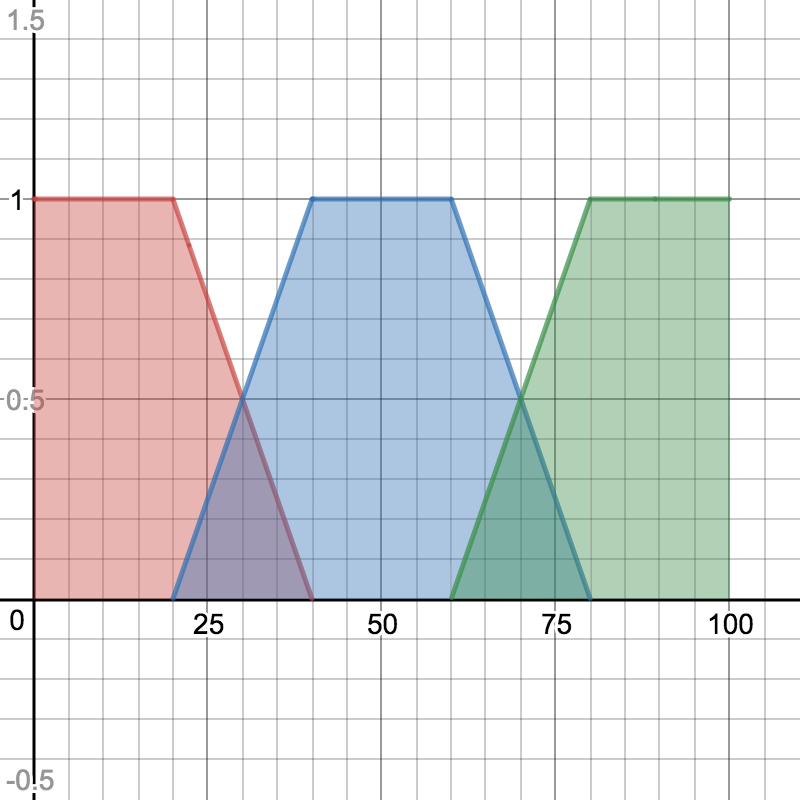
\includegraphics[width=0.9\textwidth]{fuzzy_1}
    \caption{Rappresentazioni delle classi fuzzy del numero di persone (Basso, medio e alto)}
  \end{subfigure}
  \begin{subfigure}{0.49\textwidth}
    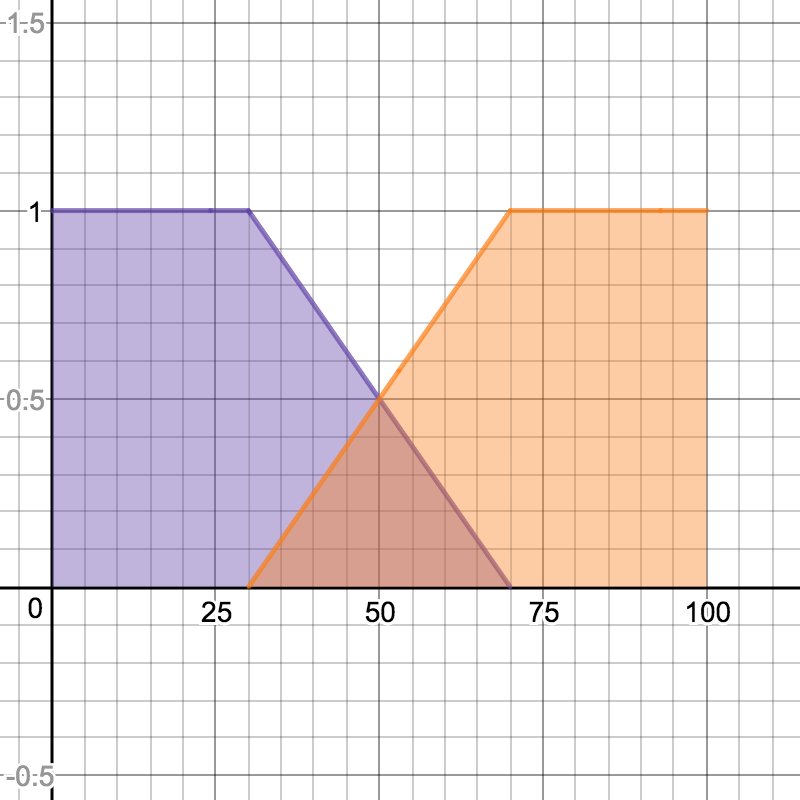
\includegraphics[width=0.9\textwidth]{fuzzy_2}
    \caption{Rappresentazioni delle classi fuzzy del carico di lavoro (leggero e pesante)}
  \end{subfigure}
\end{figure}

\subsubsection*{Variabili in uscita}
\begin{enumerate}
  \item Numero di centralinisti da attivare
        \subitem L'idea è di attivare più centralinisti quando il carico è elevato.
        \subitem Può variare da 0 a 50.
        \subitem Classificato in:
        \subsubitem Poco personale: 10 persone
        \subsubitem Personale medio: 30 persone
        \subsubitem Personale completo: 50 persone
  \item Tempo dedicabile ad ogni chiamata
        \subitem L'idea è di dedicare meni tempo se il carico di lavoro ed il numero di clienti è elevato.
        \subitem Può variare dai 5 ai 30 minuti
        \subitem Classificato in:
        \subsubitem Poco tempo: 5 minuti
        \subsubitem Medio tempo: 15 minuti
        \subsubitem Molto tempo: 30 minuti
\end{enumerate}

\subsubsection*{Costruiamo le regole della FAM per il personale}
\begin{enumerate}
  \item ALTO  $\land$ LEGGERO $=$ PERSONALE MEDIO
  \item ALTO  $\land$ PESANTE $=$ PERSONALE COMPLETO
  \item MEDIO $\land$ LEGGERO $=$ POCO PERSONALE
  \item MEDIO $\land$ PESANTE $=$ PERSONALE MEDIO
  \item BASSO $\land$ LEGGERO $=$ POCO PERSONALE
  \item BASSO $\land$ PESANTE $=$ PESONALE MEDIO
\end{enumerate}

\subsubsection*{Costruiamo le regole della FAM per il tempo}
\begin{enumerate}
  \item ALTO  $\land$ LEGGERO $=$ POCO TEMPO
  \item ALTO  $\land$ PESANTE $=$ POCO TEMPO
  \item MEDIO $\land$ LEGGERO $=$ MEDIO TEMPO
  \item MEDIO $\land$ PESANTE $=$ MEDIO TEMPO
  \item BASSO $\land$ LEGGERO $=$ MOLTO TEMPO
  \item BASSO $\land$ PESANTE $=$ MOLTO TEMPO
\end{enumerate}

\subsubsection*{Definiamo una regola di defuzzyficazione}
Utilizzo la media pesata come regola di defuzzyficazione.

\subsubsection*{Esempio: 25 persone chiamano ed il carico è al $40\%$}
25 persone in chiamata significa attivare al $50\%$ la classe BASSO, al $50\%$ la classe MEDIO e non attivare la classe ALTO.

Il carico di lavoro al $40\%$ significa attivare al $75\%$ la classe LEGGERO ed al $25\%$ la classe PESANTE.

FAM per il personale:

\begin{enumerate}
  \item ALTO=0 $\land$ LEGGERO=0.75 $=$ PERSONALE MEDIO=0
  \item ALTO=0  $\land$ PESANTE=0.25 $=$ PERSONALE COMPLETO=0
  \item MEDIO=0.5 $\land$ LEGGERO=0.75 $=$ POCO PERSONALE=0.5
  \item MEDIO=0.5 $\land$ PESANTE=0.25 $=$ PERSONALE MEDIO=0.25
  \item BASSO=0.5 $\land$ LEGGERO=0.75 $=$ POCO PERSONALE=0.5
  \item BASSO=0.5 $\land$ PESANTE=0.25 $=$ PESONALE MEDIO=0.25
\end{enumerate}

FAM per il tempo:

\begin{enumerate}
  \item ALTO=0 $\land$ LEGGERO=0.75 $=$ POCO TEMPO=0
  \item ALTO=0  $\land$ PESANTE=0.25 $=$ POCO TEMPO=0
  \item MEDIO=0.5 $\land$ LEGGERO=0.75 $=$ MEDIO TEMPO=0.5
  \item MEDIO=0.5 $\land$ PESANTE=0.25 $=$ MEDIO TEMPO=0.25
  \item BASSO=0.5 $\land$ LEGGERO=0.75 $=$ MOLTO TEMPO=0.5
  \item BASSO=0.5 $\land$ PESANTE=0.25 $=$ MOLTO TEMPO=0.25
\end{enumerate}

Eseguo la media pesante per defuzzyficare i risultati:

\[
  n_\text{centralinisti} = \frac{(0.5+0.5)*\text{POCO} + (0.25+0.25)*\text{MEDIO}}{0.5+0.5+0.25+0.25} = \frac{(0.5+0.5)*10 + (0.25+0.25)*30}{0.5+0.5+0.25+0.25} = \frac{10+15}{1.5} \approx 17
\]

\[
  n_\text{minuti} = \frac{(0.5+0.25)*\text{MEDIO} + (0.5+0.25)*\text{MOLTO}}{0.5+0.5+0.25+0.25} = \frac{(0.5+0.25)*15 + (0.5+0.25)*30}{0.5+0.5+0.25+0.25} = \frac{11.25+22.5}{1.5} \approx 23
\]

Le FAM così costruite suggeriscono quindi 17 centralinisti che dedicano 23 minuti per cliente.
\end{document}